% \pragmaonce

% adapted from https://www.overleaf.com/learn/latex/Commands
\providecommand{\dissertationelse}[2]{%
% adapted from https://tex.stackexchange.com/a/33577
\ifdefined\DISSERTATION
#1
\else
#2
\fi
}

% \pragmaonce

% adapted from https://www.overleaf.com/learn/latex/Commands
\providecommand{\dissertationexclude}[1]{%
% adapted from https://tex.stackexchange.com/a/33577
\ifdefined\DISSERTATION
\else
#1
\fi
}

% \pragmaonce

% adapted from https://www.overleaf.com/learn/latex/Commands
\providecommand{\dissertationonly}[1]{%
% adapted from https://tex.stackexchange.com/a/33577
\ifdefined\DISSERTATION%
#1%
\else%
\fi
}


\section{Methods} \label{sec:methods;ch:measuring-cna}

\subsection{Simulation}

\begin{figure}

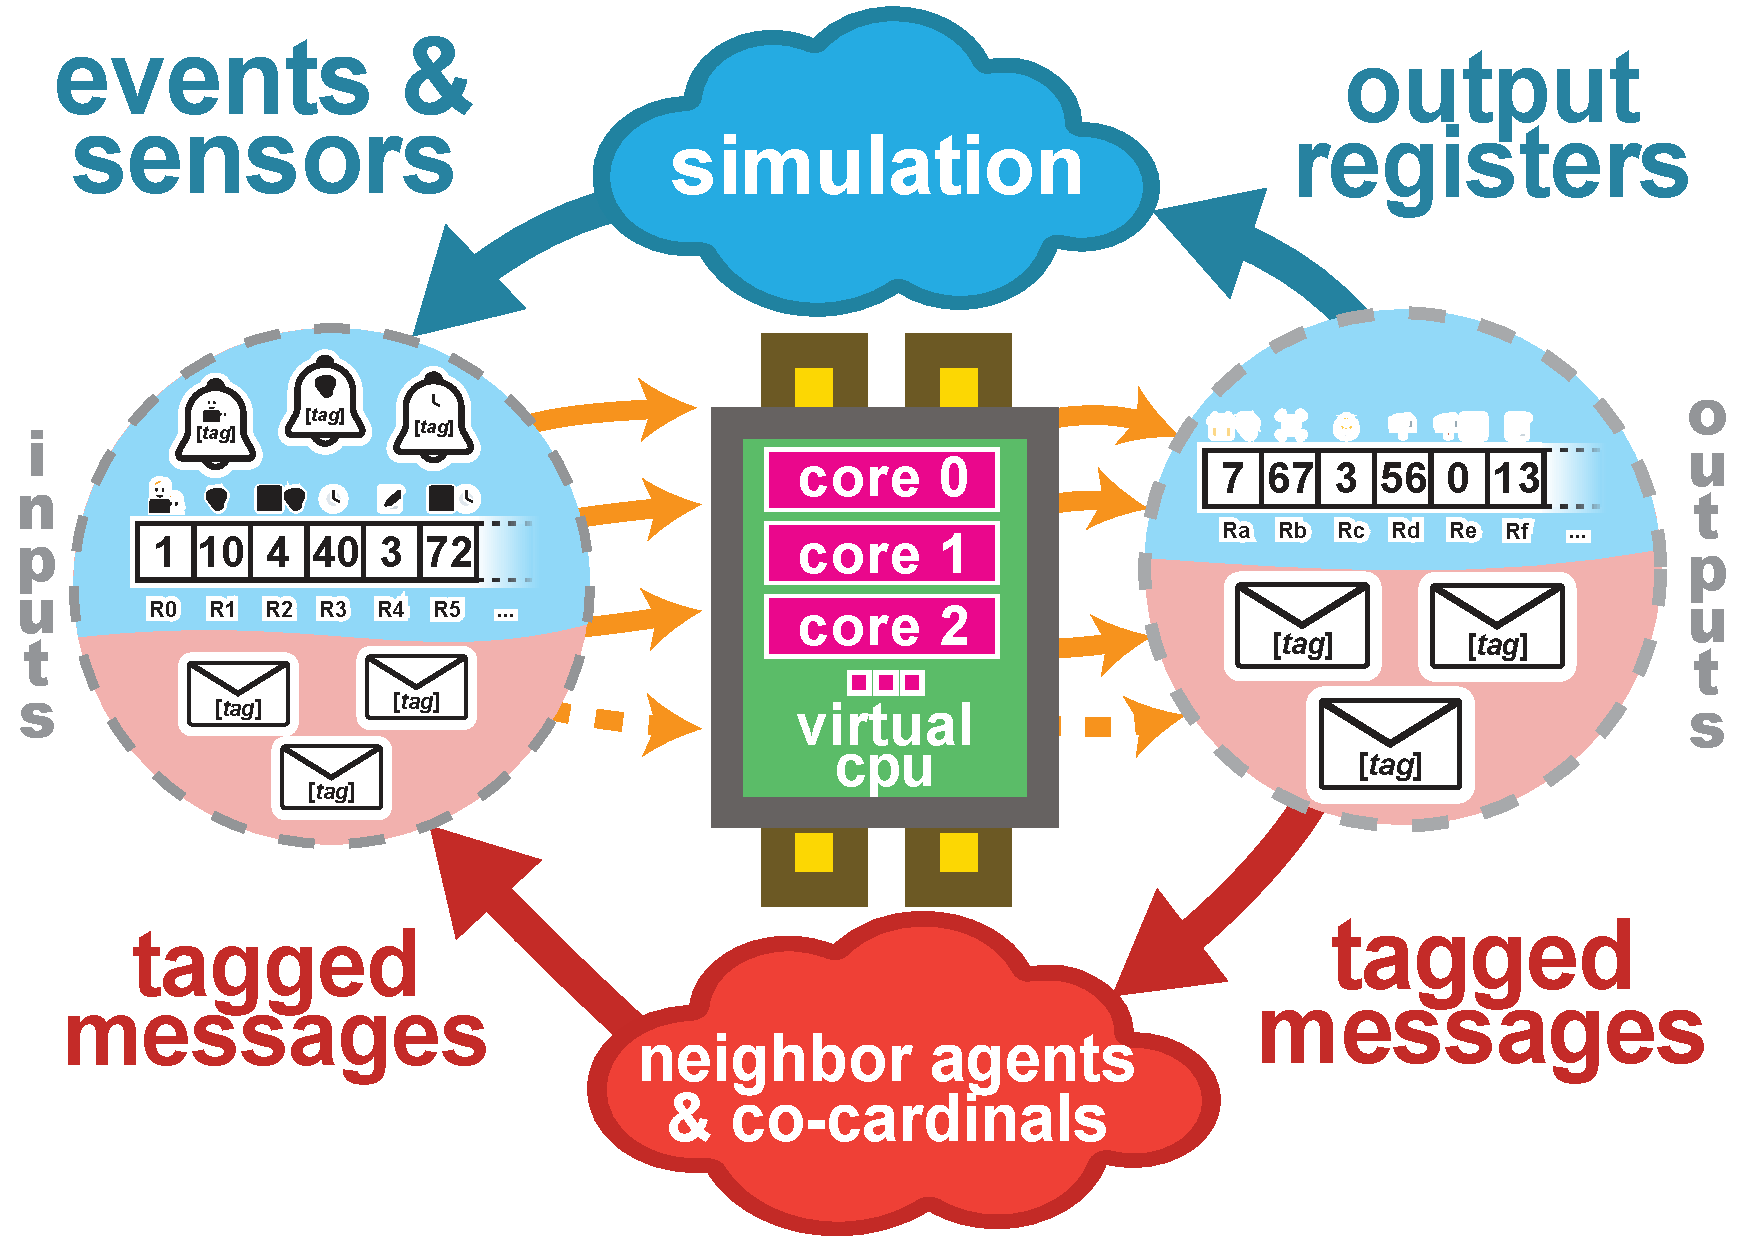
\includegraphics[width=\linewidth]{{img/cpu_detail}}

\caption{ \footnotesize
Overview of genome execution.
Tagged events and messages (shown as bells and envelopes, respectively) activate module execution on virtual cores.
Simulation state can also be read directly using sensor instructions to access input registers.
Special instructions write to output registers, allowing interaction with the simulation, and generate tagged messages, allowing interaction with other virtual CPUs.
}
\label{fig:cpu_detail}
\end{figure}


\begin{figure*}

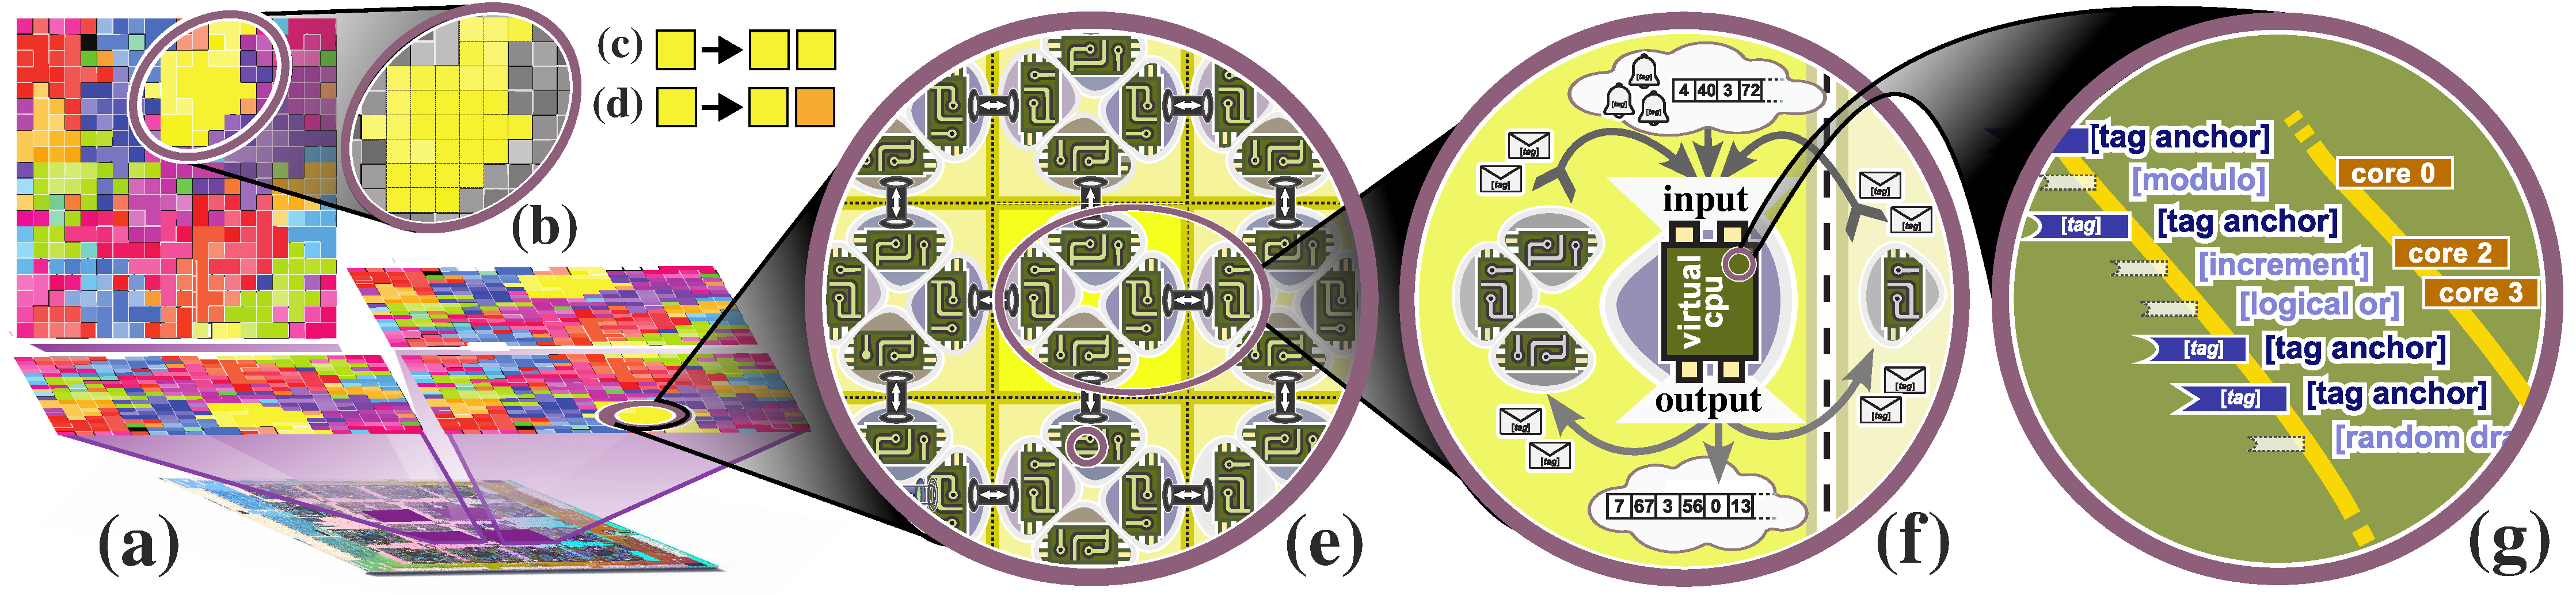
\includegraphics[width=\linewidth]{{img/graphic-oee4-cpu.pdf}}

\caption{
\textbf{Overview of digital multicell model.}
\footnotesize
Population comprises a toroidal grid of cells occupied by replicating computer programs.
In the surveyed case study, grid size was 14,400 cells ($120\times120$).
To accelerate the feasible evolutionary depth of experiments, population subgrids are evaluated across available hardware threads and processes --- in this work, 4 threads (panel $a$).
At subgrid boundaries where inter-cell interactions reach between different threads or processes, communication is handled on a best-effort basis via the underlying Conduit library.
On the population grid, cells may form local multicell groups --- shown as colored patches in visualizations (panel $b$).
Cells replicate by copying program content into a chosen neighbor cell, and may choose to grow their existing multicell group ($c$) --- or splinter their offspring off to found a new group ($d$).
Within each cell, behavior is directed by a collection of four virtual CPUs (N, S, E, and W ``cardinals''), each independently managing the cell's interactions with a one neighbor cell (panel $c$).
Each cardinal can interact with other cardinals in its own cell via message passing.
A cardinal can also exchange messages with its counterpart cardinal in the abutting neighbor cell, allowing arbitrary inter-cell communication.
Alongside message-passing I/O, cardinals accept input to sense local simulation state and create output to perform cell actions (panel $f$).
Sensory input occurs via a combination of special input registers (e.g., for own- and neighbor-cell resource availability, cell age, etc.) and special messages triggered by simulation conditions (``events,'' depicted as bells in panel $f$).
Behavior outputs are dispatched via special output registers (e.g., for resource sharing, replication, apoptosis, etc.).
At implementation level, replicator program code is evaluated via an event-driven execution model.
That is, tag-matching mechanisms trigger program submodules in response to stimuli (panel $g$).
In addition to external stimuli (i.e., inter-cellular messages, intra-cellular messages, and simulation events), program code can also trigger arbitrary self-stimuli.
Virtual hardware supports concurrent interaction handling via independent pseudo-cores, as well as dynamic plasticity through regulation of tag-matching affinities within each cardinal.
}
\label{fig:overview}
\end{figure*}


The DISHTINY simulation environment tracks cells occupying tiles on a toroidal grid (size $120\times120$ by default).
Cells collect a uniform inflow of continuous-valued resource.
This resource can be spent in increments of $1.0$ to attempt asexual reproduction into any of a cell's four adjacent cells.
A cell can only be replaced if it commands less than $1.0$ resource.
If a cell rebuffs a reproduction attempt, its resource stockpile decrements by $1.0$ down to a minimum of $0.0$.

In order to facilitate the formation of coherent multicellular groups, the DISHTINY framework provides a mechanism for cells to form groups and detect group membership \dissertationexclude{\citep{moreno2019toward}}.
Groups arise through cellular reproduction.
When a cell proliferates, it may choose to initiate its offspring as a member of its kin group, thereby growing it, or induce the offspring to found a new kin group.
This process is similar to the growth of biological multicellular tissues, where cell offspring can be retained as members of the tissue or permanently expelled.

We incentivize group formation by providing an additional resource inflow bonus based on group size.
Per-cell resource collection rate increases linearly with group size up to a cap of 12 members.
Past 12 members, the decay rate of cells' resource stockpiles begins increasing exponentially.
These mechanisms select for medium-sized groups;
the harsh penalization of oversize groups, in particular, prevents any single group from consuming the entire population.
Groups that are too small do not receive this bonus.
Groups that are too large receive a penalty.
In order to ensure group turnover, we force groups to fragment into unicells after 8,192 ($2^{13}$) updates.

% Like physical attachment in biology, these kin groups do not in and of themselves  with respect to functional individuality.
% That is, the formation of kin groups doesn't necessarily imply that constituent cells are acting as a cohesive multicellular organism (TODO cite)--- it is necessary to test for traits characteristic of multicellularity such as cooperation, coordination, and reproductive division of labor.

In \dissertationelse{Chapter \ref{ch:case-studies}}{previous work}, we established that this framework can select for traits characteristic of multicellularity, such as cooperation, coordination, and reproductive division of labor \dissertationexclude{\citep{moreno2021exploring}}.
We also found more case studies of interest arose when two nested levels of group membership were tracked
as opposed to a single, un-nested level of group membership \dissertationexclude{\citep{moreno2021exploring}}.
With nested group membership, group growth still occurs by cellular reproduction.
Cells are given the choice to retain offspring within both groups, to expel offspring from both groups, or to expel offspring from the innermost group only.
In addition to being given the choice to expel or retain offspring within both groups, cells are also allowed to expel offspring from the innermost group only.
\dissertationonly{Section \ref{sec:hierarchical_nesting} provides greater detail on group membership and hierarchical group membership in DISHTINY.}
In this work, we allow for nested kin groups.

In addition to controlling reproduction behavior, evolving genomes can also share resources with adjacent cells, perform apoptosis (recovering a small amount of resource that may be shared with neighboring cells), and pass arbitrary messages to neighboring cells.
Cell behaviors are controlled by event-driven genetic programs in which linear GP modules are activated in response to cues from the environment or neighboring agents; signals are handled in quasi-parallel on up to 32 virtual cores (Figure \ref{fig:cpu_detail}) \citep{lalejini2018evolving}.
Each cell contains four independent virtual CPUs, all of which execute the same genetic program (Figure \ref{fig:overview}a).
Each CPU manages interactions with a single neighboring cell.
We refer to a CPU managing interactions with a particular neighbor as a ``cardinal'' (as in ``cardinal direction'').
These CPUs may communicate via intra-cellular message passing.
Full details on the instruction set and event library used as well as simulation logic and parameter settings appear in supplementary material.

Supplementary Section \ref{sec:simulation-details} provides full detail on simulation components and parameters.

\subsection{Evolution}
\label{sec:evolution;ch:measuring-cna}

We performed evolution in three-hour windows for compatibility with our compute cluster's scheduling system.
We refer to these windows as ``stints.''
We randomly generated one-hundred instruction genomes at the outset of the initial stint, stint 0.
At the end of each three hour window, the system harvested and stored genomes in a population file.
We then seeded subsequent stints with the previous stint's population.
No simulation state besides genome content was preserved between stints.
In addition to simplifying implementation concerns, re-seeding each stint ensured that strains retained the capability to grow from a well-mixed innoculum.
This facilitated later competition experiments between strains.

In order to ensure heterogeneity of biotic environmental factors experienced by evolving cells, we imposed a diversity maintenance scheme.
In this scheme, descendants of a single progenitor cell from stint 0 that proliferated to constitute more than half of the population were penalized with resource loss.
The severity of the penalty increased with increasing prevalence beyond half of the population.
Thus, we ensured that descendants from at least two distinct stint 0 progenitors remained over the course of the simulation.
We arbitrarily chose a strain for primary study --- we refer to this strain as the ``focal'' strain and others as ``background'' strains.
In our case study, there was only one background strain in addition to this focal strain.

In our screen for case studies, we evolved 40 independent populations for 101 stints.
We selected population 16005 from among these 40 to profile as a case study due to its distinct asymmetrical group morphology.

At the conclusion of each stint, we selected the most abundant genome within the population as a representative specimen.
We performed a suite of follow-up analyses on each representative specimen to characterize aspects of complexity, detailed in the following subsections.
To ensure that specimens were consistently sampled from descendants of the same stint 0 progenitor, we only considered genomes with the lowest available stint 0 progenitor ID.

\subsection{Phenotype-neutral Nopout}
\label{sec:phenotype_neutral_nopout}

After harvesting representative specimens from each stint, we filtered out genome instructions that had no impact on the simulation.

To accomplish this, we performed sequential single-site ``nopouts'' where individual genome instructions were disabled by replacing them with a \texttt{Nop} instruction.
\footnote{
This \texttt{Nop} instruction was chosen to perform the same number of random number generator touches as the original instruction to control for arbitrary effects of advancing the generator.
}
We reverted nopouts that altered a strain's phenotype and kept those that did not.
To determine whether phenotypic alteration occurred, we seeded an independent, mutation-disabled simulation with the stain in question and ran it side-by-side with an independent, mutation-disabled simulation of the wildtype strain.
If any divergence in resource concentration was detected between the two strains within a 2,048 update window, the single site nopout was reverted.
We continued this process until no single-site nopouts were possible without altering the genome's phenotype.
To speed up evaluation, we performed step-by-step, side-by-side comparisons using a smaller toroidal grid size of just 100 tiles.

This process left us with a ``Phenoytpe-neutral Nopout'' variant of the wildtype genome where all remaining instructions contributed to the phenotype.
%We called the number of remaining instructions in this skeleton genome its ``phenotype complexity.''

However, in further analyses we discovered that 21 phenotype-neutral nopouts from our case study were \textit{not} actually neutral --- competition experiments revealed they were significantly less fit than the wildtype strain.
This might be due to insufficient spatial or temporal scope to observe expression of particular genome sites in our test for phenotypic divergence.
%or effects of an instruction on the mutation.

\subsection{Estimating Critical Fitness Complexity}

Next, we sought to detect genome instructions that contributed to the strain fitness.

For each remaining op instruction in the Phenotype-neutral Nopout variant, we took the wildtype strain and applied a nopout at the corresponding site.
We then competed this variant against the wildtype strain.
Evaluating only remaining op instructions in the Phenotype-neutral Nopout variant allowed us to decrease the number of fitness competitions we had to perform.

We initialized fitness competitions by seeding a population half-and-half with two strains.
We ran these competitions for 10 minutes (about 4,200 updates) on a $60\times60$ toroidal grid, after which we assessed the relative abundances of descendants of both seeded strains.

To determine whether fitness differed significantly between a wildtype and variant strain, we compared the relative abundance of the strains observed at the end of competitions against outcomes from 20 control wildtype-vs-wildtype competitions.
We fit a $T$-distribution to the abundance outcomes observed under the control wildtype-vs-wildtype competitions and deemed outcomes that fell outside the central 98\% probability density of that distribution a significant difference in fitness.
This allowed us to screen for fitness effects of single-site nopouts while only performing a single competition per site.

This process left us with a ``Fitness-noncritical Nopout'' variant of the wildtype genome where all remaining instructions contributed to the phenotype.
We called the number of remaining instructions its ``critical fitness complexity.''
We adjusted this figure downwards for the expected 1\% rate of false-positive fitness differences among tested genome sites.
This metric mirrors the MODES complexity metric described in \citep{dolson2019modes} and the approximation of sequence complexity advanced in \citep{adami2000evolution}.

% \subsection{Estimating Interpolated Fitness Complexity}

% Single-instruction nopouts  reveal sites that are critical to fitness, but are insufficient to reveal all sites that contribute to fitness.
% For example, when instructions or modules are necessary but functionally redundant, disabling only one at a time will not discover their contribution to fitness.
% Indeed, we discovered that in 97 out of the 101 representative specimens analyzed, the Fitness-noncritical Nopout variant was significantly less fit than wildtype --- clearly noncritical sites also were contributing to fitness.

% Ideally, in order to whittle down to a  ``Fitness-neutral nopout'' skeleton, we would perform a Jenga-like procedure similar to that used to arrive at the ``Phenotype-neutral nopout''.
% However, because fitness is implicit in this simulation system and must be assessed statistically through competition experiments, it is costly to assess and cannot be determined with perfect reliability.
% (Playing a large game of Jenga to completion becomes intractable if attempting to remove a piece takes more than a few seconds or you can remove a critical piece early on without realizing it.)

% Instead, we used a sampling approach and statistical inference to estimate the number of noncritical genome sites that contribute to fitness.
% We focused on the role of the $n$ instructions that were present in a strain's phenotype-neutral nopout and but absent in its fitness-noncritical nopout.
% We performed 50 fitness competitions.
% Each competition $i$ was held between a wildtype genome and the phenotype-neutral nopout with with $h_i=i\times n/50$ randomly chosen additional noncritical instructions nopped out.
% This allowed us to sample the genome space interpolated between the phenotype-neutral nopout and the fitness-noncritical nopout.

% We modeled the occurrence of deleterious fitness effect as drawing any complete set of $s$ cards from a deck totaling $n$ cards with $m$ distinct sets shuffled in among them.
% In this model, a deleterious effect manifests when a set of $s$ specific sites are nopped out together.
% The model allows for $m$ independent available sets, any of which could cause a deleterious fitness effect.
% The probability $p_d(n,m,s,h)$ of a deleterious outcome (nopping at least one complete set of interacting sites) for a specific value of $m$, $n$, and $s$ given that $h$ sites have been nopped out can be calculated exactly through a recursive formula (Supplementary Listing \ref{lst:probability_deleterious}).

% For each sampled competition, we observed either a deleterious or a neutral outcome.
% The probability of the $i$th outcome with $h_i$ sites nopped is
% \begin{align*}
% p_i(m,s) =
% \begin{cases}
%     p_d(n,m,s,h_i) & \text{if deleterious}\\
%     1 - p_d(n,m,s,h_i) & \text{if neutral}
% \end{cases}
% \end{align*}

% We can calculate the likelihood of the particular set of 50 outcomes we observed given an underlying number of sets $m$ and set size $s$ as $\prod_i p_i(m,s)$.
% This formula allows us to find the values of $m$ an $s$ that maximize likelihood and best explain our observed data.

% To our surprise, we found that in most instances a set size $s$ of 1 gave higher likelihoods of the observed data than larger set sizes.
% It appears that the redundancy that prevented these sites from being detected in the fitness-critical nopout was eliminated by the phenotype-neutral nopout.
% In the future, it may be practical to couple this approach with a exhaustive battery single-site nopouts on sites present in a strain's phenotype-neutral nopout and but
% %todo which word? and or but?
% absent in its fitness-noncritical nopout.
% However, for parsimony's sake for all further analyses in this work we fixed $s=1$.

% We took the value $m$ that gave maximum likelihood of observed interpolation competition outcomes as the estimate for the number of noncritical instructions that contribute to fitness.
% We called this ``interpolated fitness complexity.''
% (Noncritical fitness complexity might be a better term for this metric moving forward, however.)
% We used the range of $m$ that accounts for the central 95\% of likelihood density to construct a 95\% credible interval for this metric.

% However, we were unable to perform this estimate because in 21 phenotype-neutral nopouts were significantly less fit than wildtype.
% %todo fix this sentence; not sure what it should say

\subsection{Estimating State Interface Complexity}
\label{sec:estimating-state-interface-complexity;ch:measuring-cna}

In addition to estimating the number of genome sites that contribute to fitness, we measured the number of different environmental cues and the number of different output mechanisms that cells adaptively incorporated into behavior.

One possible way to take this measure would be to disable event cues, sensor instructions, and output registers one by one and test for changes in fitness.
However, this approach would fail to distinguish context-dependent input/output from merely contingent input/output.
For example, a cell might happen to depend on a sensor being set at a certain frequency but not on the actual underlying simulation information the sensor represents.

To isolate context-dependent input/output state interactions, we tested the fitness effect of swapping particular input/output states between CPUs rather than completely disabling them.
That is, for example, CPU $b$ would be forced to perform the output generated by CPU $a$ or CPU $b$ would be shown the input meant for CPU $a$.
We performed this manipulation on half the population in a fitness competition for each individual component of the simulation's introspective state (44 sensor states relating to the status of a CPU's own cell), extrospective state (61 sensor states relating to the status of a neighboring cell), and writable state (18 output states, 10 of which control cell behavior and 8 of which act as global memory for the CPU).
\footnote{
A full description of each piece of introspective, extrospective, and writable state is listed in supplementary material.
}
We deemed a state as fitness-critical if this manipulation resulted in decreased fitness at significance $p < 0.01$ using a $T$-test parameterized by 20 control wild-type vs wild-type competitions.

We describe the number of states that cells interact with to contribute to fitness as ``State Interface Complexity.''

\subsection{Estimating Messaging Interface Complexity}
\label{sec:estimating-messaging-interface-complexity;ch:measuring-cna}

In addition to estimating the number of input/output states cells use to interact with the environment, we also estimated the number of distinct intra-cellular messages cardinals within a cell use to coordinate and inter-cellular messages that cells use to coordinate.
As with state interface complexity, distinguishing context-dependent behavior from contingent behavior is critical to attaining a meaningful measurement.
For example, a cardinal might happen to depend on always receiving a inter-cellular message from a neighbor or an intra-cellular message from another cardinal.
Although meaningless, if that message were blocked, fitness would decrease.
So, instead of simply discarding messages to test for a fitness effect, we re-route messages back to the sending cardinal instead of their intended recipient.
We deemed a messages as fitness-critical if this manipulation resulted in decreased fitness at significance $p < 0.01$ using a $T$-test parameterized by 20 control wild-type vs wild-type competitions.

We refer to the number of distinct messages that cells send to contribute to fitness as ``Messaging Interface Complexity.''

We refer to the sum of State Interface Complexity, Intra-messaging Interface Complexity, and Inter-messaging Interface Complexity as ``Cardinal Interface Complexity.''

\subsection{Estimating Adaptation}
\label{sec:measuring-adaptation;ch:measuring-cna}

In order to assess ongoing changes in fitness, we performed fitness competitions between the representative focal strain specimen sampled at each stint and the focal strain population from the preceding stint.
(Recall from Section \ref{sec:evolution;ch:measuring-cna} that, due to a diversity maintenance procedure, two completely independent strains coexisted over the course of the experiment --- the ``focal'' strain selected for analysis and a ``background'' strain.)
Using the population from the preceding stint as the competitive baseline (rather than the representative specimen) ensured more focused, consistent measurement of the fitness properties of the specimen at the current stint (e.g., preventing skewed results from a sampled ``dud'' at the preceding stint).

We performed 20 independent replicates of each competition.
Competing strains were well-mixed within the full-sized toroidal grid at the outset of each competition, which lasted for 10 minutes of wall time.
This was sufficient to simulate about 8,000 updates at stint 0 and 2,000 updates at stint 100 (Supplementary Figures \ref{fig:num_updates_elapsed_heatmap}, \ref{fig:num_updates_elapsed_barplot}, and \ref{fig:num_updates_elapsed_boxplot}).
We determined that a gain of fitness had occurred if the current stint specimen constituted a population majority at the conclusion of more than 17 of those competitions, corresponding to a significance level of $p < 0.005$ under the two-tailed binomial null hypothesis.
Likewise, we deemed winning fewer than 3 competitions a significant fitness loss.


\subsection{Implementation}

We employed multithreading to speed up execution.
We split the simulation into four $60\times60$ subgrids.
Each subgrid executed asynchronously, using the Conduit C++ Library \dissertationonly{presented in Chapter \ref{ch:conduit}} to orchestrate best-effort, real-time interactions between simulation elements on different threads \dissertationexclude{\citep{moreno2021conduit}}.
This approach is inspired by Ackley's notion of indefinite scalability \citep{ackley2014indefinitely}.
In other work benchmarking the system, we have demonstrated that this approach improves scalability.
The simulation scales to 4 threads with 80\% efficiency, up to 64 threads with 40\% efficiency and up to 64 nodes with 80\% efficiency \dissertationelse{(Chapter \ref{ch:conduit})}{\citep{moreno2021conduit}}.
%TODO multicellular between distribute dsystems We are excited about the potential of the system not just

% https://mybinder.org/v2/gh/mmore500/dishtiny/e17e6d5e258b7aacac72d44922008ab14e80e182?filepath=binder%2Fbucket%3Dprq49%2Fa%3Dall_stints_all_series_profiles%2Bendeavor%3D16%2Fcase_study_16005.ipynb
Over the 101 three-hour evolutionary stints performed to evolve the case study, 7,565,309 simulation updates elapsed.
This translates to 74,904 updates elapsed per stint or about 6.9 updates per second.
However, the update processing rate was not uniform across stints: the simulation slowed about 77\% as stints progressed.
Supplementary Figure \ref{fig:simulation} shows elapsed updates for each stint.
During stint 0, 176,816 updates elapsed (about 16.3 updates per second).
During stint 100, only 41,920 updates elapsed (about 3.8 updates per second).

% https://mybinder.org/v2/gh/mmore500/dishtiny/e17e6d5e258b7aacac72d44922008ab14e80e182?filepath=binder%2Fbucket%3Dprq49%2Fa%3Dall_stints_all_thread_profiles%2Bendeavor%3D16%2Felapsed_updates.ipynb
Although working asynchronously, threads processed similar number of updates during each stint.
The mean standard deviation of update-processing rate between threads was 2\%.
The mean difference of the update-processing rate between the fastest and slowest threads was 5\%.
The maximum value of these statistics observed during a stint was 9\% and 20\%, respectively, at stint 44.
Supplementary Figure \ref{fig:simulation:thread_updates} shows the distribution of elapsed updates across threads for each stint evolved during the case study.

%TODO dependencies
